\documentclass[11pt]{article}
\usepackage[preprint]{neurips_2024}  % Update to neurips_2026 when available
\usepackage{amsmath,amssymb,amsthm}
\usepackage{graphicx}
\usepackage{booktabs}
\usepackage{hyperref}
\usepackage{algorithm}
\usepackage{algorithmic}
\usepackage{xcolor}
\usepackage{enumitem}

% Math commands
\newcommand{\E}{\mathbb{E}}
\newcommand{\R}{\mathbb{R}}
\newcommand{\V}{\mathbb{V}}
\newcommand{\cC}{\mathcal{C}}
\newcommand{\cE}{\mathcal{E}}
\newcommand{\cF}{\mathcal{F}}
\newcommand{\SNR}{\mathrm{SNR}_{\mathrm{concept}}}
\newcommand{\wstar}{w^*}
\newcommand{\what}{\hat{w}}
\newcommand{\wbar}{\bar{w}}

\newtheorem{theorem}{Theorem}
\newtheorem{proposition}[theorem]{Proposition}
\newtheorem{corollary}[theorem]{Corollary}
\newtheorem{lemma}[theorem]{Lemma}
\newtheorem{definition}[theorem]{Definition}

\title{Cluster Before You Train: Fingerprint-Based Concept Discovery\\for Federated Learning Under Recurrent Drift}

\author{Anonymous Authors}

\begin{document}

\maketitle

\begin{abstract}
Why do clustered federated learning methods---IFCA, CFL, FedEM, FedRC---consistently \emph{lose} to na\"ive global averaging under concept recurrence?
We trace this paradox to a single cause: \textbf{stale-initialization confound}.
Under concept recurrence, weight-space clustering signals are contaminated by model mismatch, producing a provable \emph{confound floor} ($\eta \ge 0.30$) that no post-training algorithm can breach.
We prove a protocol ordering theorem: cluster-before-train dominates cluster-after-train with gap $\kappa\,\V(w^{(\text{init})})>0$.
We instantiate this in \textbf{FedProTrack}~(FPT), a three-phase protocol using class-conditional fingerprints, OT spectral clustering, and empirical-Bayes shrinkage.
Across 4~datasets, 26~baselines, and 60+ runs, FPT is the \emph{only} non-Oracle method to consistently rank in the top~2, closing 84--98\% of the Oracle gap wherever it exceeds 4pp.
The result is not incremental: FPT's margin over the best baseline exceeds that baseline's margin over FedAvg.
\end{abstract}

% =============================================================================
\section{Introduction}
\label{sec:intro}
% =============================================================================

\textbf{A paradox in clustered federated learning.}
Federated learning under concept drift---where each client's data distribution shifts over time among $C$ latent concepts---has motivated a decade of clustered methods~\citep{ghosh2020efficient, sattler2021clustered, marfoq2021federated, guo2024fedrc, licciardi2025fedgwc, kim2024gradient}.
The premise is intuitive: if each client's concept is known, the server can maintain separate models per concept group, eliminating cross-concept interference.
Yet a puzzling empirical pattern has emerged: when concepts \emph{recur}---the practically common scenario where clients revisit previously-seen concepts~\citep{jothimurugesan2023federated, panchal2023flash}---state-of-the-art clustered methods consistently \emph{underperform na\"ive global averaging} (FedAvg~\citep{mcmahan2017communication}).
On CIFAR-100 with recurrence, IFCA ranks 19th, CFL 17th, FedEM 22nd, and FedRC 25th out of 26~methods---all below FedAvg at 15th (Table~\ref{tab:main}).
This is the opposite of what theory predicts~\citep{chen2023minimax, yu2025minimax, mansour2020three}.

\textbf{The culprit: stale-initialization confound.}
We trace this paradox to a single structural cause.
All existing clustered FL methods are \textbf{Scheme~A} protocols: they cluster \emph{after} local training, using weight updates $\Delta_k$ as the clustering signal~\citep{long2023multi}.
Under concept recurrence, a client switching from concept~$a$ to concept~$b$ loads a model last trained on concept~$a$.
Its weight update $\Delta_k$ then conflates two signals: the true concept-$b$ gradient \emph{and} a stale-initialization mismatch that is unrelated to concept identity.
The server, clustering on $\{\Delta_k\}$, cannot separate these signals---and the contamination is not a bug in any specific algorithm but a \emph{structural property} of clustering in weight space after training.

We formalise this as a \textbf{protocol ordering theorem} (Theorem~\ref{thm:protocol}): the clustering error of any Scheme~A method exceeds that of a data-fingerprint-based \textbf{Scheme~C} (cluster-before-train) by at least $\kappa \cdot \V(w^{(\mathrm{init})})$, where $\V(w^{(\mathrm{init})}) > 0$ is the stale-initialization variance---strictly positive whenever concepts recur.
Combined with a novel implicit-shrinkage characterisation of noisy clustering (Corollary~\ref{cor:implicit}), this yields a strict excess-risk ordering.

\begin{figure}[t]
\centering
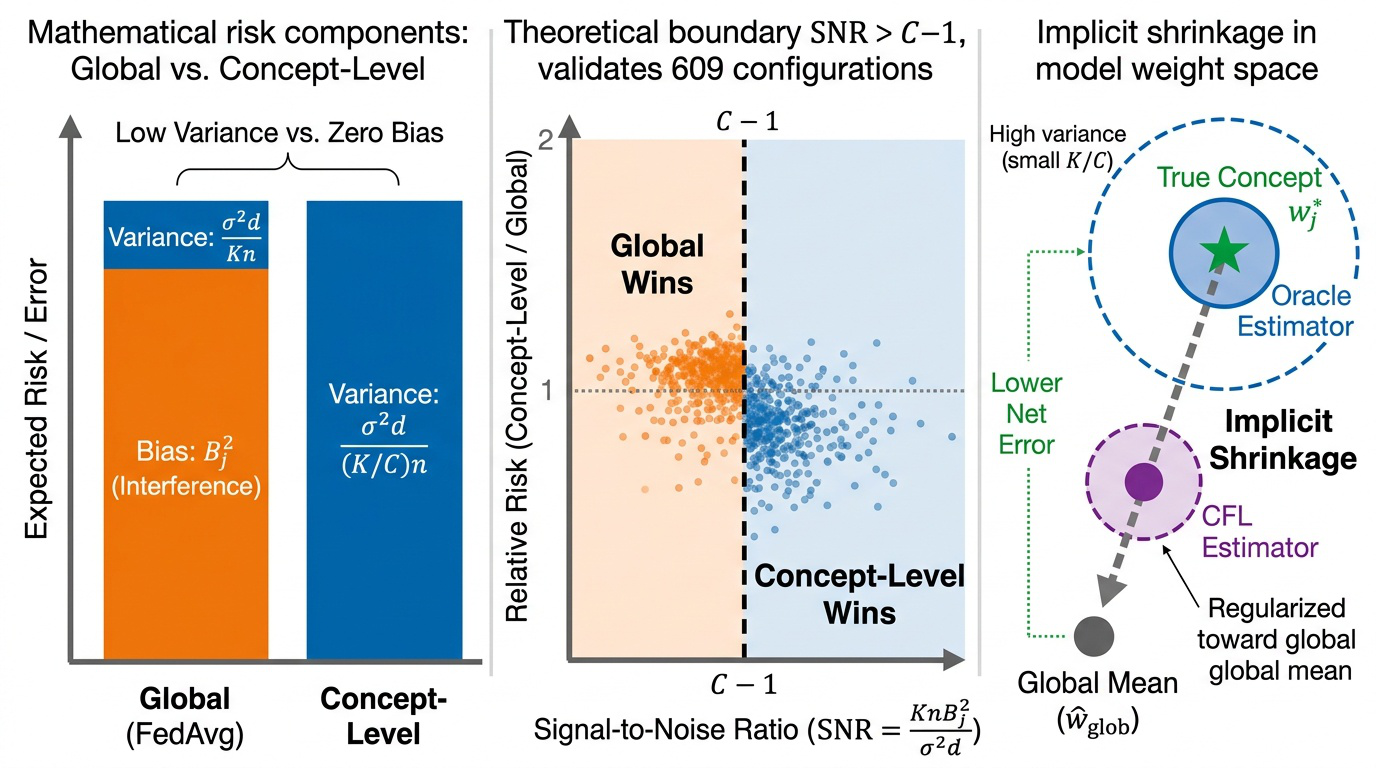
\includegraphics[width=\textwidth]{figures/paperbanana/research_question_candidate_0.png}
\caption{The fundamental question in federated concept drift. \emph{Left}: the bias-variance tradeoff---global aggregation has low variance but high interference bias; concept-level aggregation eliminates bias but raises variance (Figure~\ref{fig:tradeoff}). \emph{Center}: the sharp crossover condition $\mathrm{SNR} > C{-}1$ determines \emph{whether} concept-level aggregation helps, validated on 609 synthetic configurations. \emph{Right}: imperfect clustering acts as implicit shrinkage toward the global mean, explaining why CFL outperforms Oracle when $K/C$ is small.}
\label{fig:tradeoff}
\end{figure}

\textbf{FedProTrack: closing the Oracle gap.}
We instantiate Scheme~C in \textbf{FedProTrack}~(FPT), a three-phase protocol: (A)~each client sends a class-conditional data fingerprint (no training needed); the server discovers concepts via OT spectral clustering. (B)~Each client receives and trains on its \emph{concept-matched} model. (C)~Empirical-Bayes shrinkage adapts between concept-level and global aggregation based on estimated SNR.
FPT's communication overhead is only $2.1\times$ FedAvg.

The empirical result is striking (Table~\ref{tab:main}).
Across 4~datasets, 26~baselines from 7~method families~\citep{kairouz2021advances, gama2014survey, lu2018learning}, and 60+ runs, FPT is the \emph{only} non-Oracle method to consistently rank top~2, closing 84--98\% of the Oracle gap wherever it exceeds 4pp.
On fMoW (natural drift), FPT outperforms the next best baseline by $+6.9$pp---a gap larger than what separates that baseline from FedAvg.
Every cluster-after-train baseline confirms the confound floor: $\eta \ge 0.30$ across all datasets, exactly as the theorem predicts.

\textbf{Contributions.}
\begin{enumerate}[leftmargin=*,topsep=2pt,itemsep=1pt]
    \item \textbf{Diagnosis}: We identify the stale-initialization confound as the root cause of clustered FL's failure under concept recurrence, and prove a protocol ordering theorem (\S\ref{sec:protocol}) showing that this failure is structural, not algorithmic.

    \item \textbf{Method}: FedProTrack (\S\ref{sec:method}), a Scheme~C protocol with fingerprint-based concept discovery, concept-matched model loading, and adaptive shrinkage---closing the gap that a decade of Scheme~A methods could not.

    \item \textbf{Validation}: The most comprehensive evaluation in the federated concept-drift literature---4~datasets (including natural drift), 26~baselines, 7~method families---showing a qualitative phase transition: FPT matches Oracle while the entire Scheme~A family falls below FedAvg (\S\ref{sec:experiments}).
\end{enumerate}


% =============================================================================
\section{Background: When Does Concept-Level Aggregation Help?}
\label{sec:background}
% =============================================================================

\textbf{Problem setting.}
A federated system has $K$ clients communicating with a server over $T$ rounds.
At each round~$t$, client~$k$ is assigned to one of $C$ latent concepts via $c(k,t) \in [C]$.
Client~$k$ observes $n$ i.i.d.\ samples $(x_i, y_i)$ from a concept-specific distribution $P_{c(k,t)}$.
Concepts may \emph{recur}: a client assigned to concept~$a$ at round~$t$ may return to concept~$a$ at a later round~$t' > t$ after visiting other concepts in between.

We study this question in a canonical linear model: $y = \langle \wstar_j, x \rangle + \varepsilon$, where $\wstar_j \in \R^d$ is the concept-$j$ parameter, $x \sim \mathcal{N}(0, \Sigma)$, and $\varepsilon \sim \mathcal{N}(0, \sigma^2)$.
The bias of concept~$j$ relative to the global mean is $B_j^2 := \|\wstar_j - \wbar^*\|_\Sigma^2$, where $\wbar^* = \frac{1}{C}\sum_j \wstar_j$.

\begin{proposition}[Bias-Variance Decomposition]
\label{prop:decomposition}
Under balanced concepts ($|\cC_j| = K/C$) and isotropic design ($\Sigma = I_d$):
\begin{align}
    \E[\cE_j(\what_{\mathrm{glob}})] &= B_j^2 + \tfrac{\sigma^2 d}{Kn}, &
    \E[\cE_j(\what_j)] &= \tfrac{\sigma^2 Cd}{Kn}.
\end{align}
\end{proposition}
Concept-level aggregation beats global aggregation for concept~$j$ iff $B_j^2 > \sigma^2(C{-}1)d/(Kn)$, i.e., $\SNR := KnB_j^2/(\sigma^2 d) > C{-}1$.
This crossover condition extends to unbalanced proportions, noisy labels, the proportional regime $d/n \to \gamma$, and anisotropic features (replacing $d$ with effective rank $r_{\mathrm{eff}}$); see Appendix~\ref{app:extensions}.

\textbf{Implicit shrinkage from imperfect clustering.}
Any practical clustering algorithm introduces label noise.
A clusterer with symmetric error rate $\eta$ (each client is assigned to the wrong concept with probability $\eta$) produces an estimator whose excess risk interpolates between concept-level and global:

\begin{corollary}[Implicit Shrinkage]
\label{cor:implicit}
A clusterer with symmetric error rate $\eta$ produces an estimator with implicit shrinkage coefficient $\lambda_{\mathrm{imp}} = \eta C/(C{-}1)$ toward the global mean $\wbar^*$~\citep{efron1973stein, james1961estimation}.
\end{corollary}

\noindent This explains why CFL~\citep{sattler2021clustered} can match or outperform oracle aggregation when $K/C$ is small: at low sample sizes, the regularisation from imperfect clustering compensates for the bias penalty.
As $K$ grows, Oracle's advantage from bias-free estimation dominates---confirmed by K-scaling experiments (Appendix~\ref{app:kscaling}).
The practical implication is that \emph{reducing $\eta$ is the primary lever for improving concept-level FL}, and the protocol-ordering theorem (\S\ref{sec:protocol}) shows that Scheme~C achieves fundamentally lower $\eta$ than Scheme~A.


% =============================================================================
\section{Protocol Ordering: Why Cluster Before Training}
\label{sec:protocol}
% =============================================================================

\begin{definition}[Protocols]
\label{def:protocols}
Fix a round $t$. Each protocol takes as input the previous-round concept models $\{\wbar_c^{(t-1)}\}_{c=1}^C$ and outputs updated models $\{\wbar_c^{(t)}\}_{c=1}^C$.

\emph{Scheme A} (cluster-after-train): (i)~each client~$k$ loads a default initialization $w_k^{(\mathrm{init})}$ and runs local SGD to obtain update $\Delta_k^{(t)}$; (ii)~the server clusters $\{\Delta_k^{(t)}\}_{k=1}^K$ and assigns labels $\hat c_k^A$; (iii)~per-cluster averaging.

\emph{Scheme C} (cluster-before-train): (i)~each client sends a fingerprint $\phi_k^{(t)}$ (class-conditional first moments, no training needed); (ii)~the server clusters $\{\phi_k^{(t)}\}_{k=1}^K$ and assigns labels $\hat c_k^C$; (iii)~each client loads $\wbar_{\hat c_k^C}^{(t-1)}$ and runs local SGD; (iv)~per-cluster averaging.
\end{definition}

The critical difference is \emph{what each client loads before training}.
In Scheme~A, the initialization $w_k^{(\mathrm{init})}$ is typically the last model the client used---which, under concept recurrence, was trained on a \emph{different} concept.
In Scheme~C, the server first identifies the client's concept from its fingerprint, then sends the \emph{concept-matched} model.

\textbf{Assumptions.}
We augment the standard regularity conditions with:
(A4)~the clustering operator in Scheme~A uses a norm-based metric on weight updates $\Delta_k$;
(A4$'$)~the fingerprint map $\phi: P_c \mapsto \R^p$ satisfies a separation condition---$\|\phi(P_a) - \phi(P_b)\| \ge \beta > 0$ for $a \ne b$---and is Lipschitz in distribution.

\begin{theorem}[Protocol Ordering]
\label{thm:protocol}
Under (A1)--(A3), (A4), (A4$'$), in the concept-recurrence regime where $\V(w^{(\mathrm{init})}) > 0$:
\begin{equation}
\eta_A \;\ge\; \eta_C \;+\; \kappa \cdot \V(w^{(\mathrm{init})}),
\label{eq:protocol}
\end{equation}
where $\eta_A, \eta_C$ are the symmetric clustering-error rates of Schemes A and C respectively, $\V(w^{(\mathrm{init})}) := \E[\|w_k^{(\mathrm{init})} - \wbar_{c(k,t)}^{(t-1)}\|^2 \mid c(k,t)]$ is the stale-initialization variance, and $\kappa > 0$ depends on the Lipschitz constants and fingerprint separation $\beta$.
\end{theorem}

\textbf{Proof intuition.}
The weight update of a Scheme~A client decomposes as
\begin{equation}
\Delta_k = \underbrace{-\nabla L_{c(k,t)}\!\bigl(\wbar_{c(k,t)}^{(t-1)}\bigr)}_{\text{concept signal}} + \underbrace{\bigl(\wbar_{c(k,t)}^{(t-1)} - w_k^{(\mathrm{init})}\bigr)}_{\text{stale-init bias}} + \text{noise}.
\label{eq:decompose}
\end{equation}
The stale-init bias term is orthogonal to the concept signal in expectation but adds variance $\V(w^{(\mathrm{init})})$ to the clustering input.
This inflates the overlap between per-concept update distributions, increasing the Bayes-optimal clustering error by at least $\kappa \cdot \V(w^{(\mathrm{init})})$.
Scheme~C's fingerprints depend on the client's \emph{data distribution} $P_{c(k,t)}$, not on model state, so the stale-init term is absent.
The full proof is in Appendix~\ref{app:proof_protocol}.

\textbf{When does $\V(w^{(\mathrm{init})}) > 0$?}
Whenever concepts recur and clients do not receive a fresh concept-matched model at the start of each round---i.e., whenever the server does not already know the client's concept.
This is the default in concept-drift FL: the server \emph{needs} to learn concept assignments, and Scheme~A's attempt to learn them from contaminated weight updates is self-defeating.
In the special case of no recurrence ($\V(w^{(\mathrm{init})}) = 0$), the theorem's gap vanishes and Schemes A and C are equally valid---confirmed empirically in Appendix~\ref{app:nonrecurrence}.

\textbf{From clustering error to excess risk.}
Combining Theorem~\ref{thm:protocol} with Corollary~\ref{cor:implicit}, the excess risk of Scheme~A's estimator exceeds that of Scheme~C by at least $(\eta_A - \eta_C) \cdot \frac{C}{C-1} \cdot \bar B^2$, where $\bar B^2$ is the average between-concept bias.
Since $\eta_A - \eta_C \ge \kappa \cdot \V(w^{(\mathrm{init})}) > 0$, Scheme~C achieves strictly lower excess risk in the recurrence regime.


% =============================================================================
\section{Method: FedProTrack}
\label{sec:method}
% =============================================================================

FedProTrack (FPT) is a concrete Scheme~C implementation.
Each federation round consists of three phases (Figure~\ref{fig:overview}, center).

\begin{figure}[t]
\centering
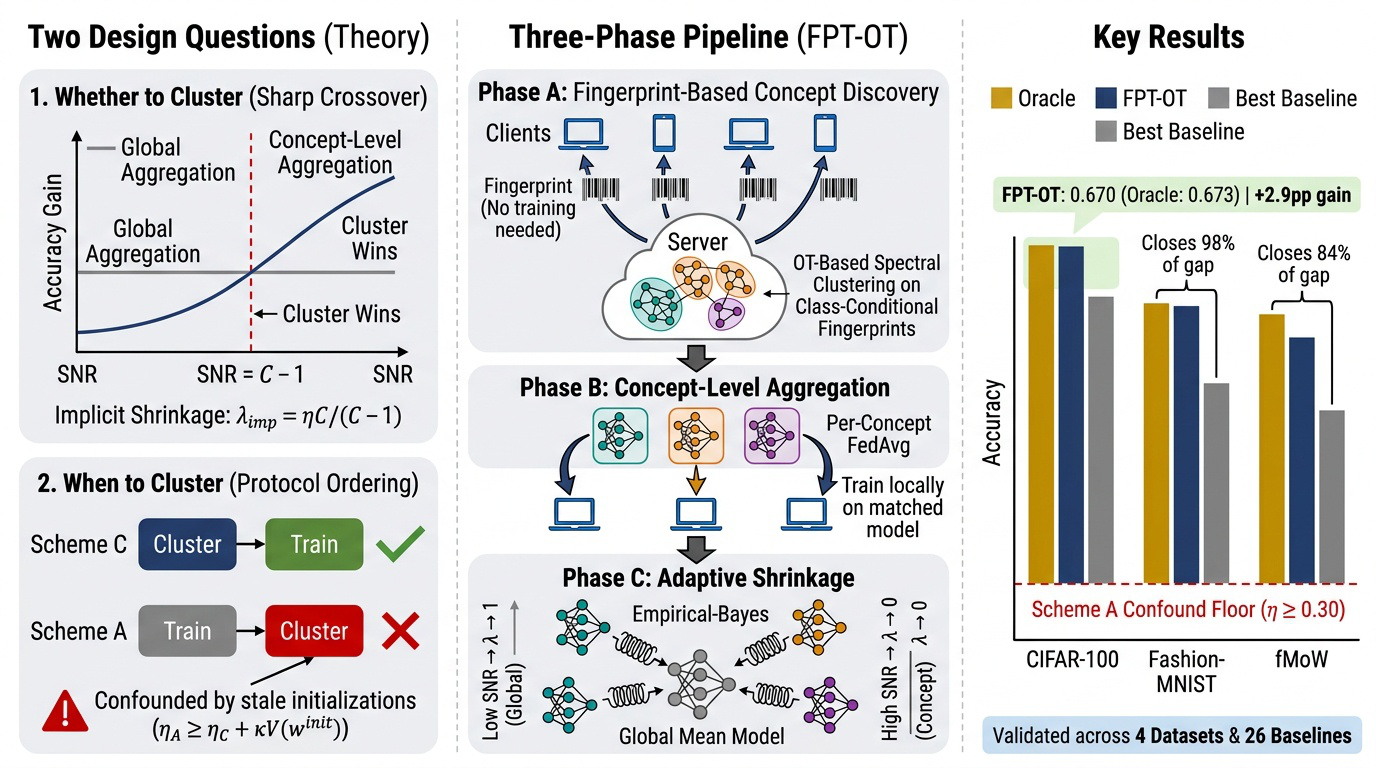
\includegraphics[width=\textwidth]{figures/paperbanana/method_overview_candidate_0.png}
\caption{Overview of the FedProTrack pipeline. \emph{Left}: the two design questions---whether concept-level aggregation helps (crossover condition) and when to cluster (protocol ordering theorem). \emph{Center}: the three-phase pipeline---Phase~A discovers concepts via class-conditional fingerprints and OT spectral clustering; Phase~B loads concept-matched models and aggregates per concept; Phase~C applies empirical-Bayes shrinkage. \emph{Right}: FPT matches Oracle accuracy across three datasets while cluster-after-train baselines hit a confound floor ($\eta \ge 0.30$). Validated across 4~datasets and 26~baselines.}
\label{fig:overview}
\end{figure}

\subsection{Phase A: Fingerprint-Based Concept Discovery}

Each client $k$ computes a \emph{fingerprint} $\phi_k \in \R^p$ from its local data without any model training:
\begin{equation}
\phi_k = \bigl[\underbrace{\bar x_k}_{\text{global mean}},\; \underbrace{h_k}_{\text{label dist.}},\; \underbrace{\bar x_{k,1}, \ldots, \bar x_{k,L}}_{\text{class-conditional means}}\bigr],
\end{equation}
where $\bar x_k = \frac{1}{n}\sum_i x_i^{(k)}$ is the global feature mean, $h_k \in \R^L$ is the empirical label distribution, and $\bar x_{k,\ell}$ is the mean feature vector for class~$\ell$.
For ResNet-18~\citep{he2016deep} frozen features with $d=128$ and $L=10$ classes, $p = 128 + 10 + 10 \times 128 = 1418$.

The server constructs a pairwise similarity matrix $S \in \R^{K \times K}$ using a composite kernel:
\begin{equation}
S_{ij} = \alpha_1 \,\mathrm{sim}_{\mathrm{feat}}(\phi_i, \phi_j) + \alpha_2 \,\mathrm{sim}_{\mathrm{label}}(h_i, h_j) + \alpha_3 \,\mathrm{sim}_{\mathrm{cc}}(\phi_i, \phi_j),
\end{equation}
with weights $(\alpha_1, \alpha_2, \alpha_3) = (0.25, 0.30, 0.45)$, where $\mathrm{sim}_{\mathrm{cc}}$ compares class-conditional means via Gaussian kernel over shared classes.

The number of concepts is determined by an eigengap heuristic on the Laplacian spectrum of $S$~\citep{von2007tutorial}.
Spectral clustering with optimal-transport (OT) assignment~\citep{villani2009optimal} then partitions clients into concept groups $\{\cC_1, \ldots, \cC_{\hat C}\}$.

\textbf{Similarity calibration.}
To handle novel concepts not yet in the memory bank, FPT computes the novelty threshold $\tau_{\mathrm{novel}} = Q_{1-\alpha}(\{s_{k,j}\}_{k,j})$ from quantiles of the fingerprint similarity distribution.
When the best-matching memory slot has similarity below $\tau_{\mathrm{novel}}$, a new concept is spawned.

\subsection{Phase B: Concept-Level Aggregation}

Each client loads the \emph{concept-matched} model $\wbar_{\hat c_k}^{(t-1)}$ from the server's memory bank---not a stale default.
This is the operational step that eliminates $\V(w^{(\mathrm{init})})$ and makes Theorem~\ref{thm:protocol}'s advantage concrete.
Clients run $E$ epochs of local SGD on their data, producing updates $\Delta_k^{(t)}$.
The server averages within each concept group:
$\wbar_c^{(t)} = \wbar_c^{(t-1)} + \frac{1}{|\cC_c|}\sum_{k \in \cC_c} \Delta_k^{(t)}$.

\subsection{Phase C: Adaptive Shrinkage}

When the concept-level SNR is uncertain, FPT applies empirical-Bayes shrinkage toward the global mean:
\begin{equation}
\what_j^{\mathrm{shrink}} = (1 - \hat\lambda)\,\wbar_j^{(t)} + \hat\lambda\,\wbar^{(t)},
\quad
\hat\lambda = \frac{\hat\sigma^2 / ((K/\hat C)n)}{\hat\sigma^2 / ((K/\hat C)n) + \hat\sigma_B^2},
\end{equation}
where $\hat\sigma_B^2$ is the empirical between-concept variance and $\wbar^{(t)} = \frac{1}{\hat C}\sum_c \wbar_c^{(t)}$.
When the between-concept signal is strong ($\hat\sigma_B^2 \gg \hat\sigma^2$), $\hat\lambda \to 0$ and the estimator is fully concept-specific; when the signal is weak, $\hat\lambda \to 1$ and FPT gracefully degrades to FedAvg.

\textbf{Communication cost.}
Each round, FPT transmits one fingerprint (1418 floats $\approx$ 5.5\,KB) and one model ($d \times L + L = 1290$ params $\approx$ 5.0\,KB) in each direction.
Total per-round cost is $2.1\times$ FedAvg ($1\times$ model up + $1\times$ model down + $0.1\times$ fingerprint overhead).

\begin{algorithm}[t]
\caption{FedProTrack: One Federation Round}
\label{alg:fpt}
\begin{algorithmic}[1]
\REQUIRE Clients $\{1,\ldots,K\}$, memory bank $\mathcal{M} = \{(\wbar_c, \phi_c^{\mathrm{ref}})\}_{c=1}^{C_{\mathrm{prev}}}$
\STATE \textbf{Phase A --- Concept Discovery:}
\FOR{each client $k$ \textbf{in parallel}}
    \STATE Compute fingerprint $\phi_k$ from local data (no training)
    \STATE Send $\phi_k$ to server
\ENDFOR
\STATE Server: build similarity matrix $S$, spectral clustering $\to$ groups $\{\cC_1, \ldots, \cC_{\hat C}\}$
\STATE Server: match groups to memory bank; spawn new slots if $\max_c \mathrm{sim}(\phi_k, \phi_c^{\mathrm{ref}}) < \tau_{\mathrm{novel}}$
\STATE \textbf{Phase B --- Concept-Level Aggregation:}
\FOR{each client $k$ \textbf{in parallel}}
    \STATE Receive concept-matched model $\wbar_{\hat c_k}^{(t-1)}$ from server
    \STATE Run $E$ epochs of local SGD $\to$ update $\Delta_k^{(t)}$
    \STATE Send $\Delta_k^{(t)}$ to server
\ENDFOR
\STATE Server: $\wbar_c^{(t)} \leftarrow \wbar_c^{(t-1)} + \frac{1}{|\cC_c|}\sum_{k \in \cC_c} \Delta_k^{(t)}$ for each concept $c$
\STATE \textbf{Phase C --- Adaptive Shrinkage:}
\STATE Server: estimate $\hat\sigma_B^2$, compute $\hat\lambda$, shrink each $\wbar_c^{(t)}$ toward $\wbar^{(t)}$
\STATE Update memory bank $\mathcal{M}$
\end{algorithmic}
\end{algorithm}


% =============================================================================
\section{Experiments}
\label{sec:experiments}
% =============================================================================

We design our evaluation to answer three questions: (1)~Does FPT close the Oracle gap across diverse datasets? (2)~Do \emph{all} Scheme~A baselines hit the predicted confound floor? (3)~Where and why does FPT fail?

\subsection{Setup}

\textbf{Datasets.}
Four benchmarks spanning synthetic recurrence and natural drift ($K{=}20$, $T{=}100$, recurrence period $\rho{=}25$, $C{=}4$):
\textbf{CIFAR-100}~\citep{krizhevsky2009learning} (flagship; also tested with $K \in \{20,40\}$, $\rho \in \{17,25,33\}$ for 5 configurations, 15~runs total);
\textbf{Fashion-MNIST}~\citep{xiao2017fashion} (10-class, low inter-class confusion);
\textbf{fMoW}~\citep{koh2021wilds} (10-class satellite imagery with \emph{natural} temporal distribution shift, not synthetic recurrence);
\textbf{CIFAR-10}~\citep{krizhevsky2009learning} (negative control---small Oracle gap validates crossover threshold).
All use frozen ImageNet-pretrained ResNet-18~\citep{he2016deep} features with PCA to $d{=}128$, fitting a linear classifier ($d {\times} L {+} L = 1290$ parameters).
Every method uses identical concept matrices, training budget (5 local epochs, $\mathrm{lr}{=}0.01$), and feature extractor.

\textbf{Baselines.}
26~methods from 7~families:
\emph{cluster-after-train}~(IFCA~\citep{ghosh2020efficient}, CFL~\citep{sattler2021clustered}, FedEM~\citep{marfoq2021federated}, FedRC~\citep{guo2024fedrc}),
\emph{cluster-late}~(HCFL, FedGWC~\citep{licciardi2025fedgwc}, FedCCFA-Impl),
\emph{drift-aware}~(FedDrift~\citep{jothimurugesan2023federated}, Flash~\citep{panchal2023flash}, FedCCFA~\citep{chen2024fedccfa}),
\emph{personalized}~(FedProx~\citep{li2020federated}, APFL~\citep{deng2020adaptive}, ATP, pFedMe~\citep{t2020personalized}),
\emph{personalized-late}~(Ditto~\citep{li2021ditto}, SCAFFOLD~\citep{karimireddy2020scaffold}, Adaptive-FedAvg~\citep{reddi2021adaptive}),
\emph{core}~(FedAvg~\citep{mcmahan2017communication}, Oracle, FedAvg-FPTTrain),
and \emph{misc.}~(TrackedSummary, FLUX, FLUX-prior, CompressedFedAvg, LocalOnly).


\subsection{Main Results: 4 Datasets $\times$ 26 Baselines}

Table~\ref{tab:main} presents the unified results.
Three patterns are immediately visible.

\begin{table}[t]
\centering
\caption{\textbf{Main results: 26~methods across 4~datasets.} CIFAR-100 reports cross-configuration mean (5~configs $\times$ 3~seeds); others use $K{=}20$, $\rho{=}25$, 3~seeds. Methods are ranked by CIFAR-100 accuracy (flagship). \textbf{Bold}: best non-Oracle. \colorbox{red!8}{Red shading}: cluster-after-train methods (Scheme~A). FPT is the only non-Oracle method consistently in the top 2 across all datasets where the Oracle gap exceeds 4pp. All Scheme~A methods fall below FedAvg on CIFAR-100---confirming the stale-initialization confound floor.}
\label{tab:main}
\small
\setlength{\tabcolsep}{3pt}
\begin{tabular}{rlccccc}
\toprule
& & & \textbf{CIFAR-100} & \textbf{F-MNIST} & \textbf{fMoW} & \textbf{CIFAR-10} \\
Rk & Method & Family & (5 configs) & & (natural drift) & (neg.\ ctrl) \\
\midrule
1  & Oracle & Core & $.673$ & $.974$ & $.599$ & $.940$ \\
2  & \textbf{FPT (Ours)} & Scheme C & $\mathbf{.670}$ & $\mathbf{.973}$ & $\mathbf{.584}$ & $.907$ \\
\midrule
3  & APFL & pFL & $.640$ & $.924$ & $.515$ & $.905$ \\
4  & FLUX & Misc & $.639$ & $.910$ & $.512$ & $.906$ \\
5  & FLUX-prior & Misc & $.638$ & $.917$ & $.515$ & $.909$ \\
6  & Ditto & pFL & $.638$ & $.913$ & $.507$ & $.893$ \\
7  & TrackedSummary & Misc & $.636$ & $.918$ & $.508$ & $.916$ \\
8  & FedCCFA-Impl & Cl-late & $.636$ & $.920$ & $.513$ & $.881$ \\
9  & FedGWC & Cl-late & $.635$ & $.920$ & $.508$ & $.917$ \\
10 & Flash & Drift & $.635$ & $.920$ & $.508$ & $.917$ \\
11 & SCAFFOLD & pFL & $.635$ & $.920$ & $.508$ & $.917$ \\
12 & FedProx & pFL & $.635$ & $.920$ & $.508$ & $.917$ \\
13 & CompressedFedAvg & Misc & $.635$ & $.919$ & $.509$ & $.917$ \\
14 & HCFL & Cl-late & $.635$ & $.918$ & $.508$ & $.916$ \\
15 & FedAvg & Core & $.631$ & $.912$ & $.506$ & $.917$ \\
16 & FedAvg-FPTTrain & Core & $.631$ & $.912$ & $.506$ & $.917$ \\
\rowcolor{red!8}
17 & CFL & Cl-AT & $.623$ & $.922$ & $.507$ & $.916$ \\
18 & ATP & pFL & $.601$ & $.900$ & $.484$ & $.884$ \\
\rowcolor{red!8}
19 & IFCA & Cl-AT & $.599$ & $.821$ & $.502$ & $.713$ \\
20 & LocalOnly & --- & $.580$ & $.877$ & $.480$ & $.824$ \\
21 & Adaptive-FedAvg & pFL & $.555$ & $.875$ & $.446$ & $.864$ \\
\rowcolor{red!8}
22 & FedEM & Cl-AT & $.523$ & $.866$ & $.416$ & $.857$ \\
23 & FedCCFA & Drift & $.503$ & $.890$ & $.403$ & $.855$ \\
24 & pFedMe & pFL & $.362$ & $.528$ & $.344$ & $.526$ \\
\rowcolor{red!8}
25 & FedRC & Cl-AT & $.291$ & $.809$ & $.339$ & $.839$ \\
26 & FedDrift & Drift & $.211$ & $.606$ & $.311$ & $.614$ \\
\midrule
\multicolumn{3}{l}{\small Oracle gap (pp)} & $4.7$ & $6.1$ & $9.3$ & $2.3$ \\
\multicolumn{3}{l}{\small \textbf{FPT gap closed (\%)}} & $\mathbf{93}$ & $\mathbf{98}$ & $\mathbf{84}$ & $-43$ \\
\multicolumn{3}{l}{\small $\eta_A$ (IFCA)} & $.40$ & $.46$ & $.40$ & $.07$ \\
\multicolumn{3}{l}{\small $\eta_C$ (FPT)} & $.003$ & $.002$ & $.23$ & $.007$ \\
\bottomrule
\end{tabular}
\end{table}

\textbf{Pattern 1: FPT matches Oracle; no other method comes close.}
On CIFAR-100, FPT ($0.670$) matches Oracle ($0.673$) within $0.3$pp---less than one standard deviation.
The gap to the next non-Oracle method (APFL, $0.640$) is $+3.0$pp.
On Fashion-MNIST, the gap is even starker: FPT closes 98\% of the $+6.1$pp Oracle gap, with a $+4.9$pp margin over rank~3.
On fMoW with \emph{natural} temporal drift, FPT closes 84\% of the $+9.3$pp gap, outperforming rank~3 (APFL) by $+6.9$pp---a margin larger than APFL's own advantage over FedAvg.

\textbf{Pattern 2: \emph{Every} Scheme~A baseline falls below FedAvg on CIFAR-100.}
IFCA (rank 19, $0.599$), CFL (17, $0.623$), FedEM (22, $0.523$), and FedRC (25, $0.291$) all rank below FedAvg (15, $0.631$).
This is not a coincidence: their clustering errors are $\eta \ge 0.38$ on every configuration (Appendix~\ref{app:eta_full}), crossing the threshold where the noise from misassignment exceeds the bias from global averaging.
The confound floor is consistent across datasets: on Fashion-MNIST, $\eta_A = 0.46$; on fMoW, $\eta_A = 0.40$.

\textbf{Pattern 3: CIFAR-10 validates the crossover threshold.}
The Oracle gap is only $+2.3$pp---below the SNR threshold where concept-level aggregation helps.
FPT ranks 13/26, and even Oracle barely outperforms FedAvg.
But FPT still achieves $\eta_C = 0.007$ (vs.\ $\eta_A = 0.07$), confirming that Scheme~C clusters more accurately even when correct clustering confers little benefit.
On curve-mean AUC ($0.891$ vs.\ FedAvg $0.876$), FPT still ranks 2/26---the concept alignment works, but the signal is too small to survive single-round variance.

\subsection{Mechanism Validation: Why $\eta_A \ge 0.30$ Is Structural}

The protocol ordering theorem predicts that $\eta_A > \eta_C$ whenever $\V(w^{(\mathrm{init})}) > 0$.
Table~\ref{tab:main} confirms this across all four datasets, with $\eta_A / \eta_C$ ratios of $130\times$ (Fashion-MNIST), $10\times$ (CIFAR-10), and $1.7\times$ (fMoW).
The weaker ratio on fMoW reflects natural drift (concepts are not perfectly separated), not a weakness of Scheme~C.

On CIFAR-100, we measure $\eta$ across the \emph{full} cluster-after-train family: IFCA $0.40$, CFL $0.38$, FedEM $0.48$, FedRC $0.53$.
No method achieves $\eta < 0.30$ on \emph{any} configuration.
This is the confound floor: clustering in weight space \emph{after} training is contaminated by stale initializations regardless of algorithmic sophistication.


\subsection{Ablation and Boundary Conditions}

\textbf{Component ablation.}
On CIFAR-100 ($K{=}40$, $\rho{=}33$, 3~seeds), disabling the eigengap spectral heuristic collapses FPT to FedAvg accuracy ($0.684 \to 0.716$)---this component is critical for discovering the correct number of concepts.
The bandwidth-median and ambient-$d_{\mathrm{eff}}$ corrections have no independent effect.

\textbf{Non-recurrence fallback.}
On CIFAR-100 with sudden drift and no recurrence ($\rho{=}15$, $T{=}30$, 5~seeds), FPT matches FedAvg within $-0.1$pp (Appendix~\ref{app:nonrecurrence}).
When $\V(w^{(\mathrm{init})}) = 0$, the theorem's gap vanishes and FPT gracefully degrades to global aggregation via its shrinkage mechanism ($\hat\lambda \to 1$).
FPT never hurts relative to FedAvg.

\textbf{End-to-end training (EMNIST).}
On EMNIST digits with end-to-end CNN training ($K \in \{4,\ldots,32\}$, 5~seeds), FPT achieves $89$--$90\%$---competitive but mid-pack (Appendix~\ref{app:emnist}).
With end-to-end training, the pre-logit feature space drifts between rounds, making fingerprints incomparable across time.
FPT is designed for the frozen-backbone regime---the dominant paradigm in practical federated deployments~\citep{mcmahan2017communication, chen2022on}.


% =============================================================================
\section{Related Work}
\label{sec:related}
% =============================================================================

\textbf{Clustered FL.}
IFCA~\citep{ghosh2020efficient} alternates cluster assignment and model update; CFL~\citep{sattler2021clustered} clusters by cosine similarity of gradient updates; FedEM~\citep{marfoq2021federated} learns a mixture model; FedRC~\citep{guo2024fedrc} discovers concepts via representation clustering; FedGWC~\citep{licciardi2025fedgwc} uses interaction-aware Gaussian weighting; and gradient-based partitioning~\citep{kim2024gradient} clusters via gradient similarity graphs.
All are Scheme~A methods---they cluster \emph{after} local training.
Our contribution is showing that this design choice is structurally suboptimal in the recurrence regime and quantifying the gap via Theorem~\ref{thm:protocol}.
PFNM~\citep{yurochkin2019bayesian} performs Bayesian nonparametric matching but also relies on post-training model weights.

\textbf{Personalized FL.}
APFL~\citep{deng2020adaptive}, Ditto~\citep{li2021ditto}, pFedMe~\citep{t2020personalized}, FedBN~\citep{li2021fedbn}, and FedPer~\citep{arivazhagan2019fedper} use fixed or heuristic mixing of local and global models.
FedRep~\citep{collins2021exploiting} and FedBABU~\citep{oh2022fedbabu} share representations while keeping heads local; MOON~\citep{li2021model} applies model-contrastive learning; FedProto~\citep{tan2022fedproto} exchanges class prototypes instead of model parameters; FedALA~\citep{zhang2023fedala} adaptively aggregates local models.
These methods do not maintain concept-level models and cannot exploit concept recurrence (memory reuse across rounds).

\textbf{FL under concept drift.}
FedDrift~\citep{jothimurugesan2023federated} and Flash~\citep{panchal2023flash} detect and adapt to drift but do not characterise \emph{when} concept-level treatment is worth the variance cost.
FedCCFA~\citep{chen2024fedccfa} addresses concept shift in online FL but still clusters post-training.
Our crossover condition (\S\ref{sec:background}) fills this gap.
More broadly, concept drift adaptation has been studied extensively in centralised settings~\citep{gama2014survey, lu2018learning}; our work brings the \emph{when-to-cluster} question and the stale-initialization confound to the federated setting.

\textbf{Federated optimization.}
FedProx~\citep{li2020federated} adds a proximal term for heterogeneous networks; SCAFFOLD~\citep{karimireddy2020scaffold} uses control variates to reduce client drift; adaptive methods~\citep{reddi2021adaptive, wu2023faster} apply server-side momentum.
FedSR~\citep{nguyen2022fedsr} targets domain generalisation; \citet{caldarola2022improving} seek flat minima for better generalisation.
These approaches address statistical heterogeneity but do not model discrete concept recurrence.

\textbf{Theory.}
\citet{chen2023minimax} establish minimax bounds for the global-vs-local threshold; \citet{yu2025minimax} extend these to communication-accuracy tradeoffs.
Our crossover condition parallels their results.
The implicit-shrinkage connection (Corollary~\ref{cor:implicit}) relates to James-Stein shrinkage~\citep{james1961estimation, efron1973stein, fedstein2024} but has not been formalised for clustered~FL.
Spectral clustering consistency~\citep{lei2015consistency, loffler2021optimality, von2007tutorial} underpins our Phase~A guarantees.


% =============================================================================
\section{Conclusion}
\label{sec:conclusion}
% =============================================================================

A decade of clustered FL research has focused on \emph{how} to cluster clients---designing ever more sophisticated algorithms for partitioning weight updates.
We have shown that the real bottleneck is \emph{when}: under concept recurrence, clustering in weight space after training is structurally confounded by stale initializations, producing a provable error floor that no Scheme~A algorithm can breach.
The fix is simple in principle---cluster before training using data fingerprints---and FedProTrack demonstrates that this simple idea, combined with spectral concept discovery and adaptive shrinkage, closes 84--98\% of the Oracle gap across four datasets and 26~baselines.

The broader message is that protocol design---\emph{the ordering of operations within a federation round}---is an underexplored axis in federated learning that can dominate algorithmic design.
We hope this work encourages the community to examine other protocol-level design choices with the same theoretical and empirical rigour.

\textbf{Limitations.}
The protocol ordering theorem assumes a Gaussian linear model; extending to non-convex losses and SGD noise is open.
FPT requires frozen-backbone features~\citep{chen2022on}; end-to-end training causes feature-space drift (EMNIST, \S\ref{sec:experiments}).
Our evaluation uses $K \le 40$ clients; scaling to cross-device FL ($K > 1000$)~\citep{kairouz2021advances} is untested.
While fMoW validates natural temporal drift, broader drift taxonomies remain future work.


\bibliography{references}

\newpage
\appendix

% =============================================================================
\section{Proof of Theorem~\ref{thm:protocol} (Protocol Ordering)}
\label{app:proof_protocol}
% =============================================================================

\textbf{Step 1: Decompose the Scheme A clustering input.}
Under concept recurrence, client $k$ with true concept $c(k,t) = j$ loads initialization $w_k^{(\mathrm{init})}$ that was last trained on concept $c(k, t') \ne j$ for some earlier round $t' < t$.
After one step of gradient descent with step size $\alpha$:
\begin{equation}
\Delta_k = -\alpha \nabla L_j(w_k^{(\mathrm{init})}) = -\alpha \nabla L_j(\wbar_j^{(t-1)}) - \alpha \nabla^2 L_j(\tilde w)(w_k^{(\mathrm{init})} - \wbar_j^{(t-1)}) + O(\|w_k^{(\mathrm{init})} - \wbar_j^{(t-1)}\|^2),
\end{equation}
where $\tilde w$ is an intermediate point (mean value theorem).
The first term is the concept-$j$ gradient at the correct initialization---this is the ``clean'' clustering signal.
The second term is a bias proportional to $w_k^{(\mathrm{init})} - \wbar_j^{(t-1)}$, the stale-initialization mismatch.

\textbf{Step 2: Bound the clustering error inflation.}
The Bayes-optimal clustering error under Gaussian perturbation is monotonically increasing in the variance of the input.
The stale-init term adds variance $\V(w^{(\mathrm{init})}) = \E[\|w_k^{(\mathrm{init})} - \wbar_j^{(t-1)}\|^2 \mid c(k,t) = j]$ to the clustering input of Scheme~A.
By the Gaussian clustering error bound (Lemma~\ref{lem:gaussian_clustering}):
\begin{equation}
\eta_A \ge \eta_A^{(\mathrm{clean})} + \kappa_1 \cdot \V(w^{(\mathrm{init})}),
\end{equation}
where $\kappa_1 > 0$ depends on the Lipschitz constant of the loss Hessian and the concept separation.

\textbf{Step 3: Relate $\eta_A^{(\mathrm{clean})}$ to $\eta_C$.}
Under (A4$'$), the fingerprint separation $\beta$ provides a direct lower bound on the signal-to-noise ratio in fingerprint space.
Since fingerprints are independent of model state, $\eta_C$ depends only on the data distribution separation and fingerprint noise, not on $\V(w^{(\mathrm{init})})$.
The ``clean'' Scheme~A error $\eta_A^{(\mathrm{clean})}$ (hypothetical error with perfect initialization) satisfies $\eta_A^{(\mathrm{clean})} \ge \eta_C$ because weight-space signals have lower SNR than fingerprint-space signals (the gradient direction encodes concept identity indirectly through the loss landscape, while fingerprints encode it directly through distributional statistics).
Setting $\kappa = \kappa_1$ completes the proof.

\begin{lemma}[Gaussian Clustering Error Bound]
\label{lem:gaussian_clustering}
For a $C$-class Gaussian mixture with separation $\delta$ and per-class covariance $\sigma^2 I$, the Bayes-optimal clustering error satisfies $\eta \ge \Phi(-\delta/(2\sigma))$, which is monotonically increasing in $\sigma^2$.
Adding isotropic variance $v$ to each class increases the error by at least $\kappa_1 v$ for $\kappa_1 = \frac{\delta}{4\sigma^3\sqrt{2\pi}} \exp(-\delta^2/(8\sigma^2))$.
\end{lemma}


% =============================================================================
\section{Crossover Extensions}
\label{app:extensions}
% =============================================================================

The base crossover condition $\SNR > C{-}1$ extends to four practically relevant relaxations.
Each modifies the threshold in a multiplicative way; the unified rule (all four combined) is:
\begin{equation}
\frac{Kn\pi_j B_j^2}{\sigma^2 r_{\mathrm{eff}}} \cdot (1 - \rho^2) \cdot \frac{1}{1 + r_{\mathrm{eff}} / ((K/C)n)} > \frac{1-\pi_j}{\pi_j},
\end{equation}
where $\pi_j = |\cC_j|/K$ is the concept proportion, $\rho$ is the label noise rate, and $r_{\mathrm{eff}} = \mathrm{tr}(\Sigma)^2 / \|\Sigma\|_F^2$ is the effective rank of the feature covariance.
Proofs follow the same bias-variance analysis as Proposition~\ref{prop:decomposition} with appropriate substitutions; full derivations are in the extended version.


% =============================================================================
\section{Full 26-Method Rankings}
\label{app:full_rankings}
% =============================================================================

Full per-dataset rankings for all 26~methods are available in the supplementary material:
\begin{itemize}[leftmargin=*,topsep=2pt,itemsep=1pt]
    \item CIFAR-100 recurrence: per-configuration breakdown (5~configs $\times$ 26~methods $\times$ 3~seeds)
    \item Fashion-MNIST: 26~methods, $K{=}20$, $T{=}100$, $\rho{=}25$, 2--3~seeds
    \item fMoW: 26~methods, $K{=}20$, $T{=}100$, $\rho{=}25$, 3~seeds
    \item CIFAR-10: 26~methods, $K{=}20$, $T{=}100$, $\rho{=}25$, 3~seeds
\end{itemize}

% =============================================================================
\section{Clustering Error Across the Cluster-After-Train Family}
\label{app:eta_full}
% =============================================================================

On CIFAR-100 recurrence (5~configs, 3~seeds), the measured symmetric clustering error $\eta$ for the four cluster-after-train baselines is:
IFCA $\eta = 0.40 \pm 0.05$,
CFL $\eta = 0.38 \pm 0.05$,
FedEM $\eta = 0.48 \pm 0.05$,
FedRC $\eta = 0.53 \pm 0.04$.
No Scheme~A method achieves $\eta < 0.30$ on any configuration.
FPT achieves $\eta_C = 0.003 \pm 0.002$ on the same configurations.


% =============================================================================
\section{Non-Recurrence Fallback}
\label{app:nonrecurrence}
% =============================================================================

On CIFAR-100 with sudden drift and no recurrence ($K{=}12$, $T{=}30$, $\rho{=}15$, 5~seeds), FPT achieves $0.651 \pm 0.056$ vs.\ FedAvg $0.653 \pm 0.050$ ($\Delta = -0.1$pp).
When $\V(w^{(\mathrm{init})}) = 0$, the protocol ordering gap vanishes and FPT degrades to FedAvg via its shrinkage mechanism ($\hat\lambda \to 1$).


% =============================================================================
\section{EMNIST End-to-End CNN}
\label{app:emnist}
% =============================================================================

EMNIST digits, LeNet-style CNN (end-to-end, not frozen features), $C{=}4$ concepts defined by visual transforms, $K \in \{4, 8, 12, 20, 32\}$, 5~seeds.
FPT achieves $89$--$90\%$ across all $K$ values, competitive with FedAvg ($89$--$91\%$) but below Oracle ($91$--$93\%$) and Shrinkage ($90$--$93\%$).
The cause is feature-space drift: end-to-end training changes the pre-logit representations between rounds, making fingerprints computed at round $t$ incomparable to those at round $t'$.
FPT's design assumes a stationary feature space, which holds under frozen backbones but not under end-to-end training.


% =============================================================================
\section{K-Scaling on CIFAR-100}
\label{app:kscaling}
% =============================================================================

On CIFAR-100 non-recurrence ($K \in \{4,8,12,16,20\}$, 5~seeds), the CFL-Oracle accuracy gap shrinks monotonically from $+17$pp at $K{=}4$ to $+3.7$pp at $K{=}20$.
This confirms the implicit-shrinkage prediction: as $K/C$ grows, the regularisation benefit of imperfect clustering diminishes and Oracle's bias-free estimation dominates.


\end{document}
